\documentclass[11pt,a4paper]{article}
\usepackage{fontspec,xeCJK}
\IfFontExistsTF{Microsoft JhengHei}{
  \setCJKmainfont{Microsoft JhengHei}
  \setCJKsansfont{Microsoft JhengHei}
  \setCJKmonofont{Microsoft JhengHei}
}{
  \setCJKmainfont{Noto Serif CJK TC}
  \setCJKsansfont{Noto Sans CJK TC}
  \setCJKmonofont{Noto Sans CJK TC}
}
\usepackage[margin=22mm,headheight=15pt]{geometry}
\usepackage{amsmath,amssymb,graphicx,booktabs,longtable,array,xcolor,hyperref,listings,fancyhdr}
\definecolor{accent}{HTML}{173C57}
\hypersetup{colorlinks=true,linkcolor=accent,urlcolor=accent,pdftitle={DIC16 - Pass Transistors and Transmission Gates}}
\setlength{\parindent}{0pt}
\setlength{\parskip}{5pt}
\setlength{\emergencystretch}{3em}
\renewcommand{\arraystretch}{1.2}
\lstset{basicstyle=\ttfamily\small,breaklines=true,columns=fullflexible,frame=single}
\pagestyle{fancy}
\fancyhf{}
\fancyhead[L]{\small DIC16 / Supplied model}
\fancyhead[R]{\small Laboratory report}
\fancyfoot[C]{\thepage}
\title{\color{accent}DIC16\\[4pt]Pass Transistors and Transmission Gates}
\author{Specification-based laboratory report}
\date{17 October 2026}
\usepackage[american]{circuitikz}
\usetikzlibrary{arrows.meta,positioning,calc,shapes.geometric}
\begin{document}
\maketitle
\begin{center}\small\textbf{English edition}\\
HSPICE S-2021.09 \quad | \quad Model library supplied separately
\end{center}
\section{Objectives}

Following handout PDF pages 65--73, reconstruct MOS/TG charging and discharging, six pass chains, DC current trajectories, floating-node retention, and a transmission-gate full adder. The comparisons address threshold-limited levels, distributed RC, the loading cost of restoration, and finite retention.

\section{Handout requirements and test mapping}

\begin{center}
\small
\setlength{\tabcolsep}{4pt}
\begin{tabular}{p{.42\linewidth}p{.29\linewidth}p{.18\linewidth}}
\toprule
Requirement & Deck prefix and conditions & Status \\
\midrule
Step 1: six charge/discharge cases in Tables 16.1/16.2 & 01; 20 fF, 10 ns & Measured \\
Step 2: six four-switch chains, with/without a midpoint inverter & 02; 0.2 ns edges & Both directions measured \\
Q1: current trajectory as output voltage changes & 03; DC 0--1 V & Measured \\
Q2: TG hold over microseconds & 04; 25/115 C, 20 us & Measured \\
Q3: full adder and both output delays & 05; 8 vectors, 5 fF & 8/8; delays measured \\
\bottomrule
\end{tabular}
\end{center}

\section{Circuit and derivation}

For an NMOS passing high, $V_{GS}$ decreases as the output rises, giving the approximate cutoff $V_o\simeq V_{DD}-V_T(V_{SB})$. A PMOS passing low retains a residual level near $|V_{TP}|$. Body effect changes threshold with node voltage, so a constant-threshold straight line is inadequate. Parallel N/P paths in a TG complement each other for high and low transfer.

Chains 1/2 use PMOS, 3/4 NMOS, and 5/6 TGs. Even-numbered chains add an inverter between switches 2 and 3, reversing their input-to-output polarity relative to odd-numbered chains. The first two PMOS devices in chain 6 use $L=0.6\,\mu$m, following the visible entries in the scanned Table 16.3; other dimensions are explicit in the deck. This asymmetry and scan ambiguity are retained rather than silently replacing every length by $0.25\,\mu$m.

The adder implements the logic of Fig. 16.3 with TG multiplexers. With $P=A\oplus B$, $S=P\oplus C$ and $C_{out}=\overline P B+PC$. Sum and Carry each have one output inverter; complemented data is generated before the TGs so the final inversion is included correctly. This is an explicitly documented logic-equivalent TG implementation; its delay is not claimed to reproduce the scanned schematic's internal parasitics exactly.

\section{Simulation setup and interpretation}

The supplied encrypted MOS model is evaluated at a baseline supply of 1.0 V and 25\,$^\circ$C. The 1.0 V value is a teaching condition, not a verified voltage rating. These results do not reproduce the handout's original process or supply conditions. Unless stated in the deck, $W_n/W_p/L=0.6/1.8/0.25\,\mu\mathrm m$, bulks are tied to their corresponding rails, and output load is 5 fF. Transmission-gate and weak-feedback dimensions are specified explicitly in each deck.

PrimeSim HSPICE S-2021.09 win64 was used with \texttt{RUNLVL=6}, \texttt{ACCURATE}, and \texttt{WARNLIMIT=100}. Every baseline and \texttt{.alter} analysis concluded without errors or failed measurements. The simulator still reports suppressed warnings associated with encrypted blocks; this does not establish that the model is warning-free or that those warnings are harmless. The \texttt{.tran} print interval is not a fixed integration step: the solver uses adaptive timesteps. A finite sweep is not a complete process qualification.

Unless stated otherwise, the declared functional diagnostic uses $V\leq0.2$ V for low and $V\geq0.8$ V for high. These are report-level interpretation thresholds, not numerical handout requirements or extracted receiver noise margins. Correct samples do not exclude glitches between samples. Figures are redrawn from actual simulation data; \texttt{results/} contains per-case waveforms, measurements, and derived comparison CSV files.

Public decks omit model loading paths; model configuration is added only to local execution copies. The model itself is not distributed. The first two filename digits identify the deck numbers used below. Every deck is standalone.

\section{Results}

\subsection{End levels and chain delay}

\begin{center}
\small
\setlength{\tabcolsep}{4pt}
\begin{tabular}{lr}
\toprule
Path & Voltage at 10 ns (V) \\
\midrule
PMOS charge & 1.000001 \\
PMOS discharge & 0.347873 \\
NMOS charge & 0.642986 \\
NMOS discharge & 0.000004 \\
TG charge & 1.000003 \\
TG discharge & 0.000004 \\
\bottomrule
\end{tabular}
\end{center}

\begin{figure}[htbp]
\centering
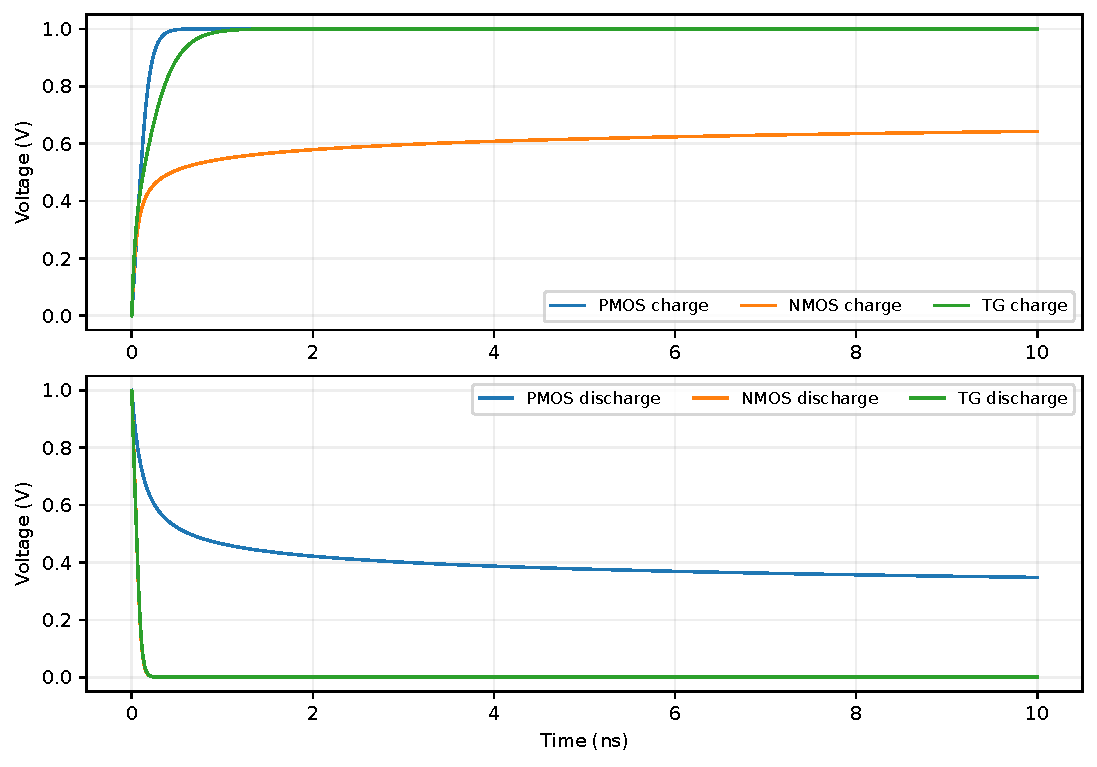
\includegraphics[width=.96\linewidth]{figures/pass_device_levels.pdf}
\caption{Six initialized capacitor charge/discharge cases; the weak transfer direction of a single MOS does not reach the full rail.}
\end{figure}

\begin{center}
\small
\setlength{\tabcolsep}{4pt}
\begin{tabular}{lrr}
\toprule
Chain & Input-rise delay (ns) & Input-fall delay (ns) \\
\midrule
1 & 5.2722 & 0.6198 \\
2 & 3.1878 & 2.3384 \\
3 & 0.2843 & 1.9191 \\
4 & 1.1735 & 1.4468 \\
5 & 0.4430 & 0.9402 \\
6 & 0.7254 & 1.1440 \\
\bottomrule
\end{tabular}
\end{center}

Delay is the difference between corresponding input and output 50\% crossings; the output edge is reversed for even-numbered chains. The input-rise delay of PMOS chain 1 is 5.2722 ns versus 3.1878 ns with midpoint restoration in chain 2, while the other direction becomes slower. A midpoint inverter therefore does not necessarily accelerate both transitions.

\begin{figure}[htbp]
\centering
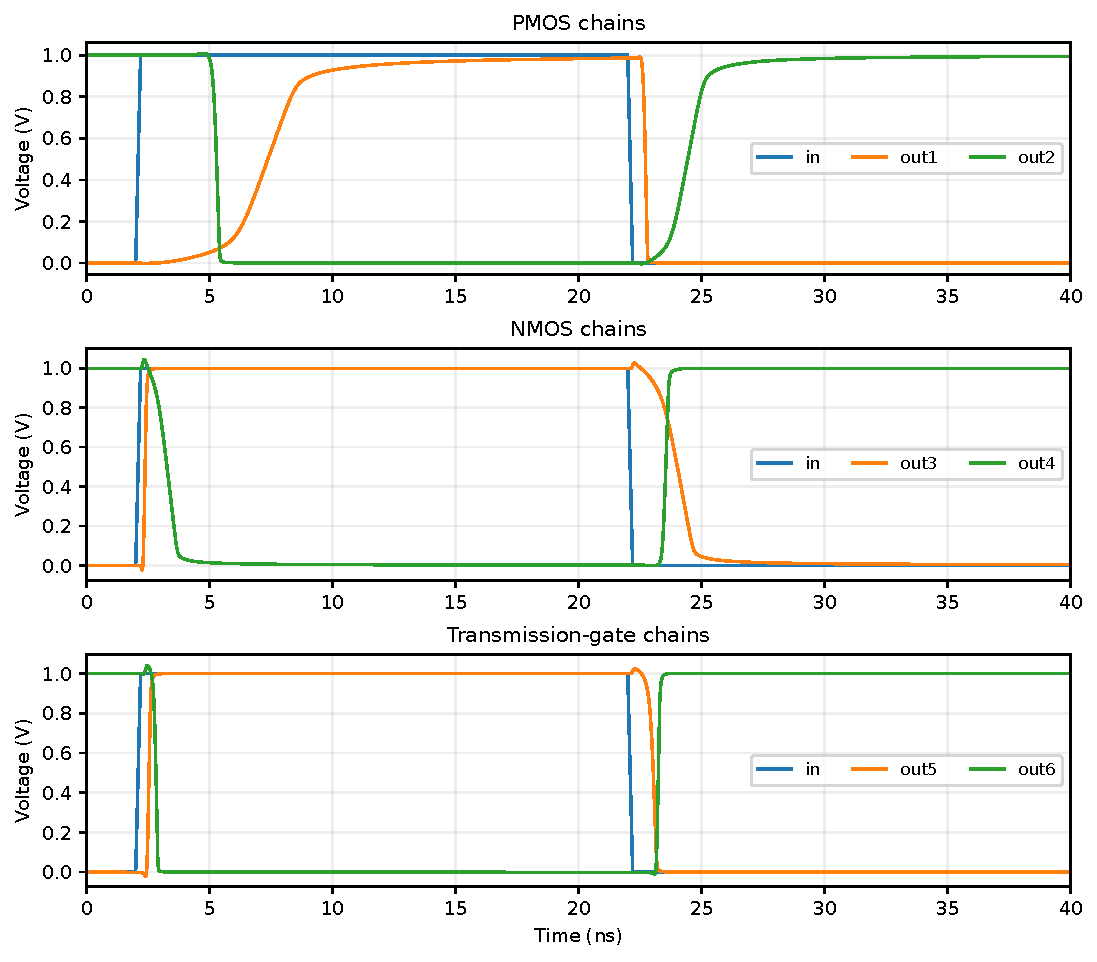
\includegraphics[width=.96\linewidth]{figures/six_chains.pdf}
\caption{Input and output waveforms of all six chains; midpoint-inverter chains have opposite output polarity.}
\end{figure}

\subsection{DC current and dynamic retention}

\begin{figure}[htbp]
\centering
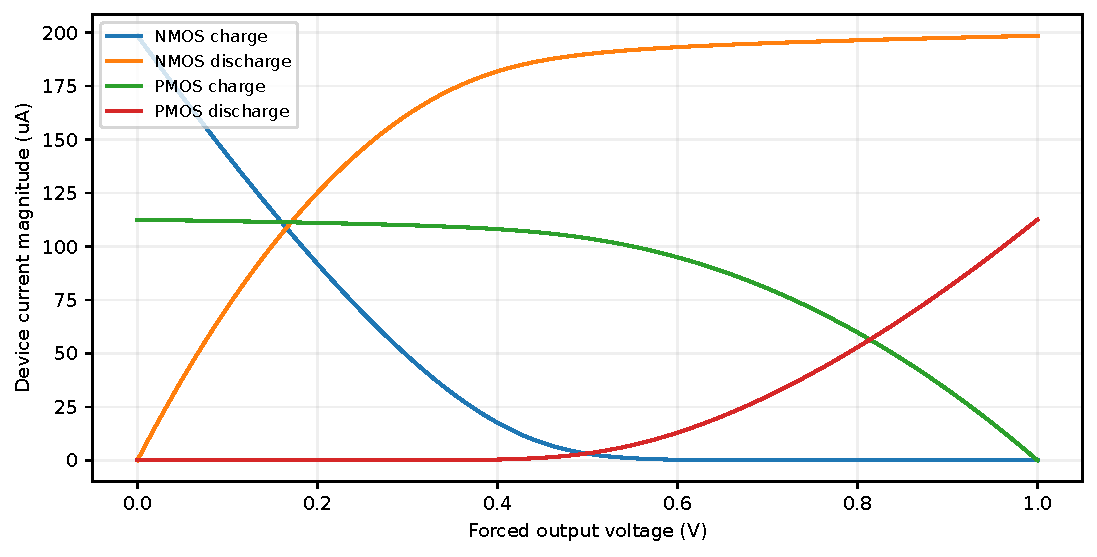
\includegraphics[width=.96\linewidth]{figures/current_trajectories.pdf}
\caption{Forced output sweep from 0 to 1 V, showing charge/discharge current trajectories for four single-MOS paths.}
\end{figure}

At an output of 0.5 V, NMOS charge/discharge currents are 3.0819/189.9322\,$\mu$A and PMOS currents are 103.8178/3.2356\,$\mu$A, directly showing their opposite weak-transfer directions. A floating node obeys $C\,dV/dt=-I_{\rm net}(V,T)$; retention must be defined against an acceptable voltage.

\begin{center}
\small
\setlength{\tabcolsep}{4pt}
\begin{tabular}{lrrrr}
\toprule
Temp. (C) & Initial (V) & 5 us (V) & 20 us (V) & To 0.8 V (us) \\
\midrule
25 & 1.0372 & 0.8926 & 0.6496 & 9.868 \\
115 & 1.0385 & 0.5252 & 0.0001 & 2.076 \\
\bottomrule
\end{tabular}
\end{center}

\begin{figure}[htbp]
\centering
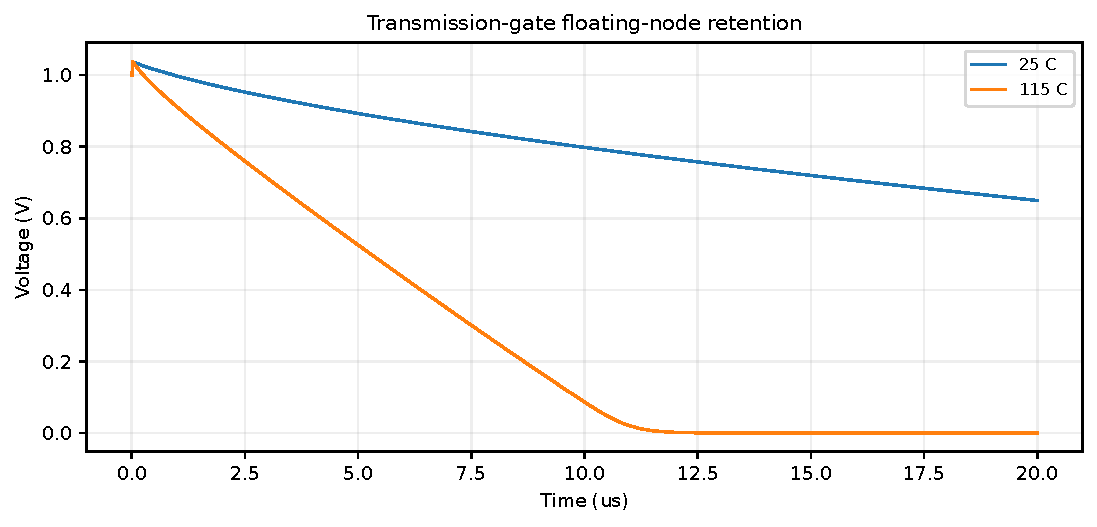
\includegraphics[width=.96\linewidth]{figures/retention.pdf}
\caption{Retention of the 20 fF node after the TG opens; the initial value slightly above 1 V is clock feedthrough.}
\end{figure}

If a node floats for half a period, the tabulated $t_{0.8}$ gives the estimate $f\gtrsim1/(2t_{0.8})$. Practical refresh needs margin and depends on the receiver threshold, load, and temperature. A single retention test does not establish a universal minimum clock frequency.

\subsection{Full adder}

\begin{center}
\small
\setlength{\tabcolsep}{4pt}
\begin{tabular}{lrrr}
\toprule
ABC & Expected S/C & Sum (V) & Carry (V) \\
\midrule
000 & 0/0 & 0.00000 & 0.00000 \\
001 & 1/0 & 1.00000 & 0.00000 \\
010 & 1/0 & 1.00000 & 0.00000 \\
011 & 0/1 & 0.00000 & 1.00000 \\
100 & 1/0 & 1.00000 & 0.00000 \\
101 & 0/1 & 0.00000 & 1.00000 \\
110 & 0/1 & 0.00000 & 1.00000 \\
111 & 1/1 & 1.00000 & 1.00000 \\
\bottomrule
\end{tabular}
\end{center}

All eight vectors give the correct settled logic. For the sensitized transition A=0, B=1, with Cin rising at 30 ns, Sum falling delay is 171.814 ps and Carry rising delay is 177.449 ps. These are the two paths under the stated vector, not worst-case delays over all vector transitions.

\begin{figure}[htbp]
\centering
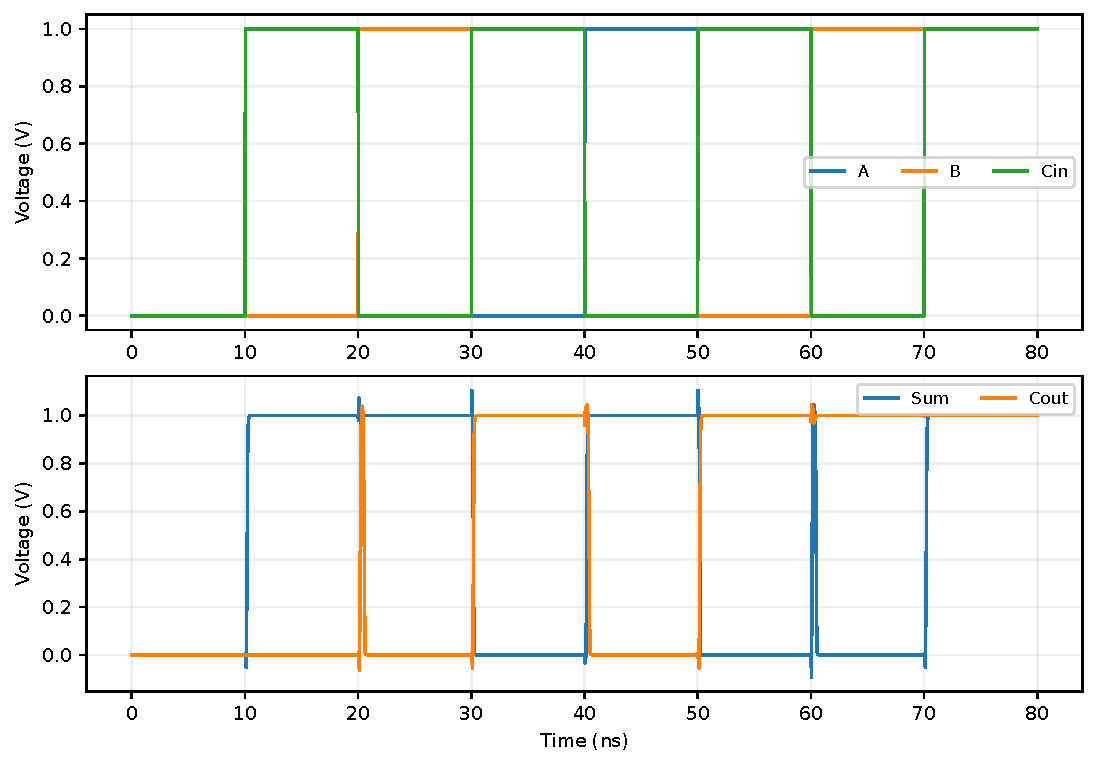
\includegraphics[width=.96\linewidth]{figures/adder.pdf}
\caption{All eight adder vectors and the Sum/Carry outputs.}
\end{figure}

\section{Discussion, differences, and unverified scope}

The original files were treated as references; independent tests were rebuilt from the handout, including DC trajectories, retention, and the full truth table. Initial conditions, loads, and chain polarity are explicit. A finite-time single-MOS endpoint is not a precise threshold extraction, and TGs still have resistance, parasitic coupling, and leakage. The complete CSV files permit alternative receiver thresholds or delay vectors.

\clearpage\section{MOS transistor schematic}
\begingroup\small
Source netlist: \texttt{01\_charge\_discharge.sp}. Complete six-branch pass-device charge/discharge test.

Identical node labels denote electrical connections. The drawings are editable CircuitikZ source; hierarchical boxes below refer to the MOS cells shown here.

Unless explicitly labeled otherwise, every NMOS body connects to \texttt{vn}=0 and every PMOS body to \texttt{vp}=\(V_{DD}\); body wires are omitted for readability. Ordinary inverter and dynamic/clocked cells use \(W_n/L_n=0.6/0.25\,\mu\mathrm m\), \(W_p/L_p=1.8/0.25\,\mu\mathrm m\). Both TG devices use \(W/L=0.6/0.25\,\mu\mathrm m\). 

\noindent\begin{minipage}[t]{.48\linewidth}\centering
\begin{circuitikz}[scale=0.85, transform shape, font=\small]
\node[nmos] (MNC) at (0,0) {};
\draw (MNC.G) -- ++(-.65,0) node[left] {\texttt{vdd}};
\node[right=3pt] at (MNC.right) {\texttt{MNC}};
\draw (MNC.S) -- ++(0,-0.8) node[below] {\texttt{vdd}};
\draw (MNC.D) -- ++(1.7,0) coordinate (o) node[above] {\texttt{nc}} to[C,l=$20\,\mathrm{fF}$] ++(0,-1.6) node[ground] {};
\end{circuitikz}
\par\small NMOS charging.
\end{minipage}\hfill\begin{minipage}[t]{.48\linewidth}\centering
\begin{circuitikz}[scale=0.85, transform shape, font=\small]
\node[nmos] (MND) at (0,0) {};
\draw (MND.G) -- ++(-.65,0) node[left] {\texttt{vdd}};
\node[right=3pt] at (MND.right) {\texttt{MND}};
\draw (MND.S) -- ++(0,-0.8) node[below] {\texttt{0}};
\draw (MND.D) -- ++(1.7,0) coordinate (o) node[above] {\texttt{nd}} to[C,l=$20\,\mathrm{fF}$] ++(0,-1.6) node[ground] {};
\end{circuitikz}
\par\small NMOS discharging.
\end{minipage}\par\medskip
\noindent\begin{minipage}[t]{.48\linewidth}\centering
\begin{circuitikz}[scale=0.85, transform shape, font=\small]
\node[pmos] (MPC) at (0,0) {};
\draw (MPC.G) -- ++(-.65,0) node[left] {\texttt{0}};
\node[right=3pt] at (MPC.right) {\texttt{MPC}};
\draw (MPC.S) -- ++(0,0.8) node[above] {\texttt{vdd}};
\draw (MPC.D) -- ++(1.7,0) coordinate (o) node[above] {\texttt{pc}} to[C,l=$20\,\mathrm{fF}$] ++(0,-1.6) node[ground] {};
\end{circuitikz}
\par\small PMOS charging.
\end{minipage}\hfill\begin{minipage}[t]{.48\linewidth}\centering
\begin{circuitikz}[scale=0.85, transform shape, font=\small]
\node[pmos] (MPD) at (0,0) {};
\draw (MPD.G) -- ++(-.65,0) node[left] {\texttt{0}};
\node[right=3pt] at (MPD.right) {\texttt{MPD}};
\draw (MPD.S) -- ++(0,0.8) node[above] {\texttt{0}};
\draw (MPD.D) -- ++(1.7,0) coordinate (o) node[above] {\texttt{pd}} to[C,l=$20\,\mathrm{fF}$] ++(0,-1.6) node[ground] {};
\end{circuitikz}
\par\small PMOS discharging.
\end{minipage}\par\medskip
\noindent\begin{minipage}[t]{.48\linewidth}\centering
\begin{circuitikz}[scale=0.88, transform shape, font=\small]
\node[nmos] (MN) at (0,0) {};
\draw (MN.G) -- ++(-.65,0) node[left] {\texttt{en}};
\node[right=3pt] at (MN.right) {\texttt{MN}};
\node[pmos,yscale=-1] (MP) at (3.4,0) {};
\draw (MP.G) -- ++(-.65,0) node[left] {\texttt{eb}};
\node[right=3pt] at (MP.right) {\texttt{MP}};

\draw (MN.D) -- ++(0,.8) coordinate (nt) -- (nt -| MP.D) -- (MP.D);
\draw (MN.S) -- ++(0,-.8) coordinate (nb) -- (nb -| MP.S) -- (MP.S);
\node[above] at ($(nt)!.5!(nt -| MP.D)$) {\texttt{b}};
\node[below] at ($(nb)!.5!(nb -| MP.S)$) {\texttt{a}};

\end{circuitikz}
\par\small TG cell: parallel NMOS and PMOS.
\end{minipage}\hfill\begin{minipage}[t]{.48\linewidth}\centering
\begin{center}\small\begin{tabular}{ll}\toprule
Instance & (a,b,en,eb)\\\midrule
\texttt{XTC} & \texttt{(vdd,tc,vdd,0)}\\
\texttt{XTD} & \texttt{(0,td,vdd,0)}\\
\bottomrule\end{tabular}\end{center}
\(C_{tc}=C_{td}=20\,\mathrm{fF}\)\par\small Both capacitors connect from the output to 0.
\end{minipage}\par\medskip
Here \(V_{DD}=1\) V. Initial conditions are \(nc=pc=tc=0\) V and \(nd=pd=td=1\) V. All gates remain enabled during the 10 ns test. Source and drain labels above follow the SPICE instance order; the body rail remains fixed even when the pass-device terminal is connected to the opposite supply.
\endgroup

\end{document}
